\chapter{Experiments and results}
This section discusses the experiment conducted and the corresponding results obtained.\\
Note: These results may vary from machine to machine.
\section{Experiment}
The idea for the experiment has been inspired from two research papers popular in the field of Face verification - ArcFace and LinCos(Cited in Bibliography). The idea is to use ArcFace but linearize cos($\theta$+m) using Taylor's expansion. This may reduce overfitting in the model obtained by training modified ArcFace model as per the idea laid down in LinCos paper.
\section{Parameter settings}
Here, we are linearizing cos($\theta$ + m) with $\sum_{n=0}^{\infty}(-1)^{n} \frac{x^{2 n}}{(2 n) !}$ (Here, x= $\theta$+m). Apart from parameters used in normal ArcFace, we can use n as another parameter. The coefficients of different terms in Taylor's expansion may be regarded as another hyper-parameters. We trained the model for n=4 and approximated cos($\theta$+m) with $1-x^2/\alpha+x^4/\beta$. Ideally, $\alpha$ and $\beta$ must be considered hyper-parameters and changed during training as per the validation loss. However, due to limitation of computational power, we directly use $\alpha=2$ and $\beta=33$. This guess has been made by comparing graphs of cos($\theta$+m) and $1-x^2/\alpha+x^4/\beta$ for different values of $\alpha$ and $\beta$. Values $\alpha=2$ and $\beta=33$ gave the best approximation for cosine.\\
\begin{figure}[!h]
    		\centering
    		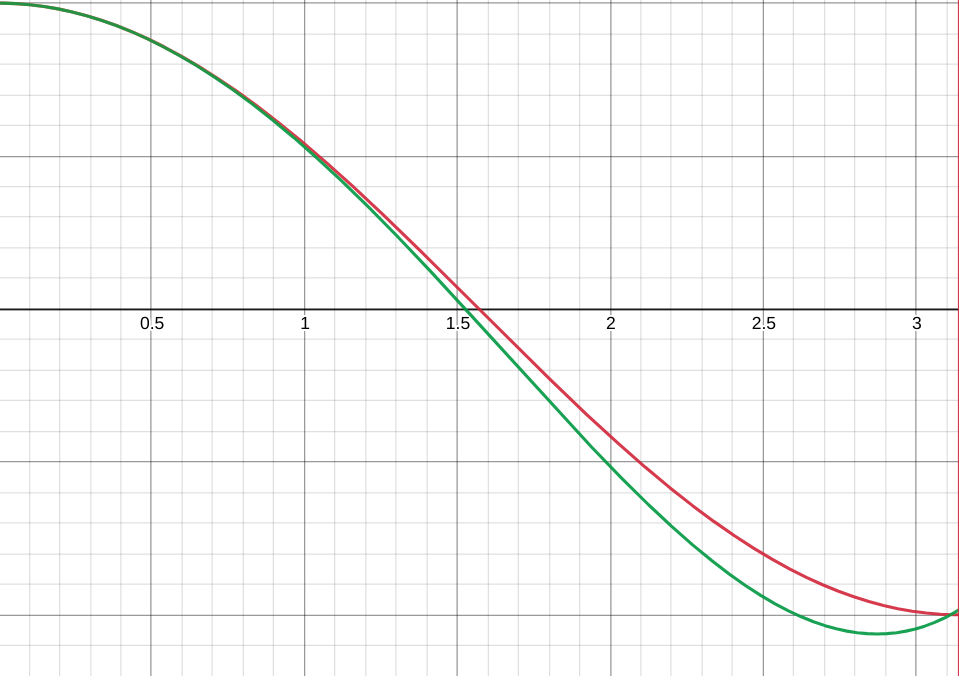
\includegraphics[width=\textwidth]{graph}
    		\caption{Graph: Red: cos(x) and green: $1-x^2/2+x^4/33$ for $0<=x<\pi$}
\end{figure}\\
List of hyper-parameters and values used during training:
\begin{itemize}
    \item n = 4 (Power of highest order term in Taylor's expansion)
    \item $\alpha$ = 2
    \item $\beta$ = 33
    \item m = 0.5 (Marginal Penalty)
    \item net\_mode = mobilefacenet ([ir, ir\_se, mobilefacenet])
    \item net\_depth = 50
    \item drop\_ratio = 0.6
    \item lr = 0.001 (Learning rate)
    \item momentum = 0.9
    \item max\_epochs = 100 (Early stopping enabled)
\end{itemize}
\section{Experiment description}
First, we train the pre-trained model with ArcFace head without any modifications on the LFW dataset(Labelled Faces in the wild). Then, the pre-trained model is trained using modified ArcFace head with above-stated parameters. After that, the results of both the models are compared based on accuracy obtained on validation and test sets.
\section{Results and discussion}
The results obtained from the models have been stated in the table below:
\begin{center}
\begin{tabular}{ |c|c|c|c| } 
\hline
Model & Accuracy\_train & Accuracy\_test & Training\_time on AWS p2.xlarge instance \\
\hline
ArcFace & $96.883\%$ & $97.0\%$ & 15.2 hours(Approx.) \\ 
\hline
ArcFace Modified & $97.4\%$ & $97.683\%$ & 10.13 hours(Approx.) \\ 
\hline
\end{tabular}
\end{center}\\
**Testing has been done using LFW benchmark.\\
It can be seen that Accuracy increases marginally. However the point to note is that, training time reduces drastically. This may be attributed to more linearity in the model produced by Taylor's expansion. However, there is a scope of mode research to find the exact reason to this drastic decline in training time.
\\
\begin{figure}[!h]
    		\centering
    		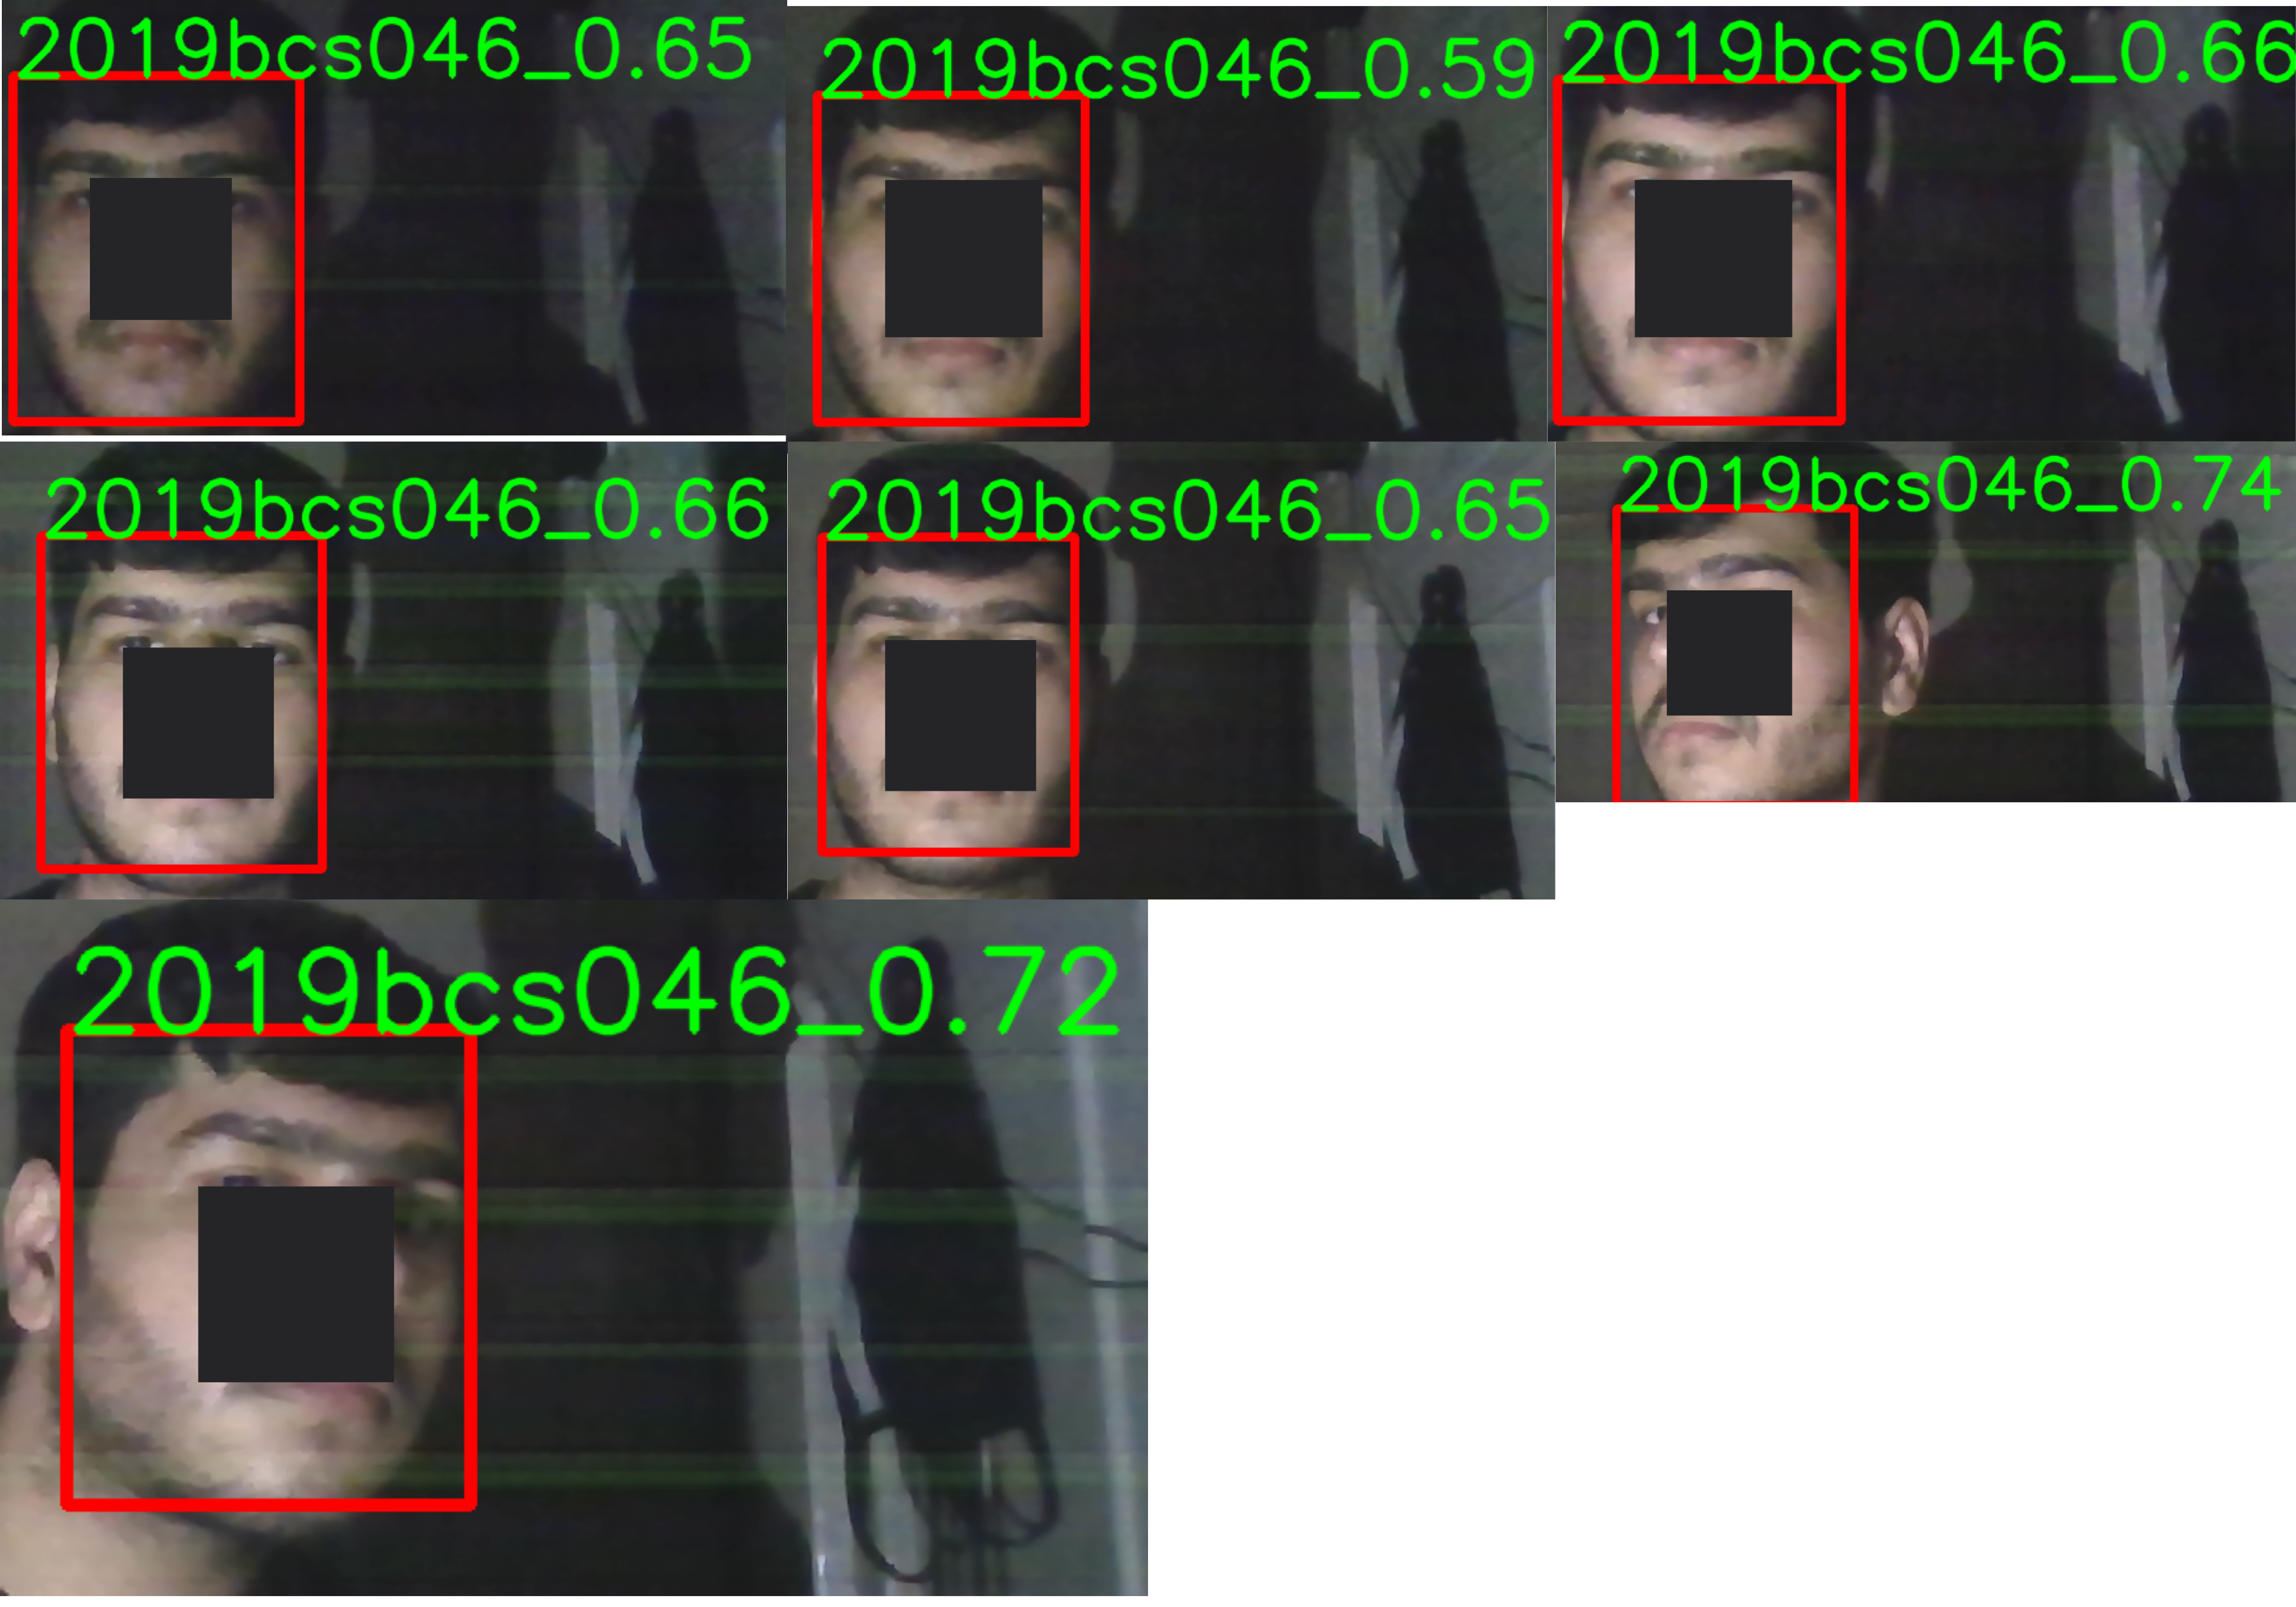
\includegraphics[width=\textwidth]{test}
    		\caption{Model testing for varying brightness and orientation}
\end{figure}\\

\section{Conclusion}
The results are not enough to conclude that modified ArcFace performs better than the original model. There needs to be more rigorous testing. 